\documentclass{article}
\usepackage{tikz}
\usepackage{amsmath}

\begin{document}

\begin{center}
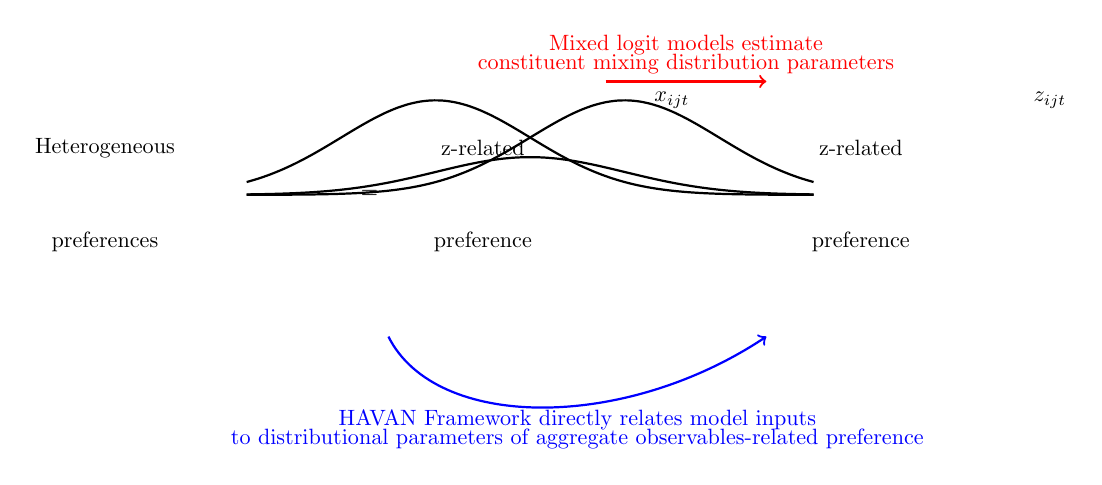
\begin{tikzpicture}[scale=1.2, every node/.style={scale=0.8}]
    % Draw the leftmost bell curve
    \draw[domain=-3:3,smooth,variable=\x, samples=50, thick] plot ({\x},{exp(-((\x)^2)/2)/(sqrt(2*pi))});
    \node at (-4.5,.5) {Heterogeneous};
    \node at (-4.5,-.5) {preferences};

    % Draw the equality sign
    \node at (-1.7,0) {$=$};

    % Draw the two bell curves representing z-related preferences
    \draw[domain=-3:3,smooth,variable=\x, samples=50, thick] plot ({\x},{exp(-((\x-1)^2)/2)});
    \node at (-0.5,.5) {z-related};
    \node at (-0.5,-.5) {preference};

    \draw[domain=-3:3,smooth,variable=\x, samples=50, thick] plot ({\x},{exp(-((\x+1)^2)/2)});
    \node at (3.5,.5) {z-related};
    \node at (3.5,-.5) {preference};

    % Draw the 'x_ijt' and 'z_ijt' labels
    \node at (1.5,1) {$x_{ijt}$};
    \node at (5.5,1) {$z_{ijt}$};

    % Draw the red arrow and annotation
    \draw[->, red, thick] (0.8,1.2) -- (2.5,1.2);
    \node[above, red] at (1.65,1.4) {Mixed logit models estimate};
    \node[above, red] at (1.65,1.2) {constituent mixing distribution parameters};

    % Draw the blue arrow and annotation
    \draw[->, blue, thick] (-1.5,-1.5) .. controls (-1, -2.5) and (1, -2.5) .. (2.5,-1.5);
    \node[below,blue] at (.5,-2.2) {HAVAN Framework directly relates model inputs};
    \node[below,blue] at (.5,-2.4) {to distributional parameters of aggregate observables-related preference};

\end{tikzpicture}
\end{center}

\end{document}